\begin{figure}
    \centering
    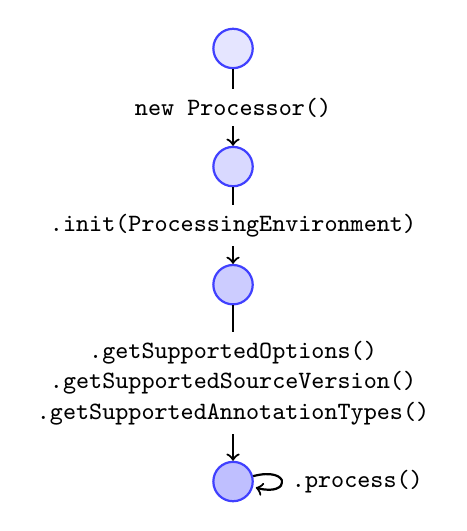
\begin{tikzpicture}
        \tikzstyle{edge-node}=[font=\small\ttfamily, align=center, fill=white]
        \tikzstyle{node}=[circle, thick, draw=black, minimum size=5mm]
        \tikzstyle{transition}=[->, thick]
        % \draw (0, -2) grid (6, 2);
        \node[node, draw=blue!75, fill=blue!10] (start) at (0, 0) {};
        \node[node, draw=blue!75, fill=blue!15] (processor) at (0, -1.5) {};
        \node[node, draw=blue!75, fill=blue!20] (processor-init) at (0, -3) {};
        \node[node, draw=blue!75, fill=blue!25] (processor-gets) at (0, -5.5) {};
        % \node[node] (process) at (0, -7.5) {};

        \draw[transition] (start) -- node[edge-node] {new Processor()} (processor);
        \draw[transition] (processor) -- node[edge-node] {.init(ProcessingEnvironment)} (processor-init);
        \draw[transition] (processor-init) -- node[edge-node] {.getSupportedOptions()\\.getSupportedSourceVersion()\\.getSupportedAnnotationTypes()} (processor-gets);
        \draw[transition] (processor-gets) edge[loop right] node[edge-node] {.process()} (processor-gets);

    \end{tikzpicture}
    \caption{Java's annotation processor lifecycle.}
    \label{fig:java-annotation-processor}
\end{figure}